\documentclass[a4paper]{article}
\usepackage[
	top=1.25in,
	bottom=1.25in,
	left=0.75in,
	right=0.75in
]{geometry}
\usepackage{tikz}
\usepackage{pgfplots}
\usepackage{amsmath}
\usepackage{amsfonts}

% Used to allow [cc|c] in     \begin{pmatrix}[cc|c]...\end{pmatrix}
\makeatletter
\renewcommand*\env@matrix[1][*\c@MaxMatrixCols c]{%
	\hskip -\arraycolsep
	\let\@ifnextchar\new@ifnextchar
	\array{#1}
}
\makeatother

\begin{document}
	\begin{enumerate}
		\item
		\begin{enumerate}
			\item
			\begin{align*}
				(2-3i) \times (1 + 5i) &=  2(1 + 5i) - 3i(1 + 5i) \\
				&= 2 + 10i - 3i + 15 \\
				&= 17 + 7i
			\end{align*}
			
			\item
			\begin{align*}
				\left( \tfrac{1}{3} - \tfrac{3}{8}i \right) \times \left( \tfrac{1}{2} + \tfrac{1}{7}i \right) &=  \tfrac{1}{3} \left( \tfrac{1}{2} + \tfrac{1}{7}i \right) - \tfrac{3}{8}i \left( \tfrac{1}{2} + \tfrac{1}{7}i \right) \\
				&= \tfrac{1}{6} + \tfrac{1}{21}i - \tfrac{3}{16}i + \tfrac{3}{56} \\
				&= \tfrac{37}{168} - \tfrac{47}{336}i
			\end{align*}
		\end{enumerate}
		
		\item
		\begin{enumerate}
			\item 
			\begin{align*}
				r &= \sqrt{0^2 + 1^2} = 1 \\
				\theta &= \frac{\pi}{2} \\
				z &= 1 \angle \tfrac{\pi}{2}
			\end{align*}
			
			\item 
			\begin{align*}
				r &= \sqrt{(\sqrt{3})^2 + 3^2} = 2 \sqrt{3} \\
				\theta &= \arctan \left( \tfrac{-3}{\sqrt{3}} \right) = - \tfrac{\pi}{3} \\
				z &= 2 \sqrt{3} \angle \tfrac{5 \pi}{3}
			\end{align*}
			
			\item 
			\begin{align*}
				r &= \sqrt{3^2 + (\sqrt{3})^2} = 2 \sqrt{3} \\
				\theta &= \arctan \left( \tfrac{\sqrt{3}}{3} \right) = \tfrac{\pi}{6} \\
				z &= 2 \sqrt{3} \angle \tfrac{\pi}{6}
			\end{align*}
			
			\item 
			\begin{align*}
				r &= \sqrt{3^2 + (\sqrt{3})^2} = 2 \sqrt{3} \\
				\theta &= \arctan \left( \tfrac{\sqrt{3}}{3} \right) + \pi = \tfrac{7 \pi}{6} \\
				z &= 2 \sqrt{3} \angle \tfrac{7 \pi}{6}
			\end{align*}
			
			\item 
			\begin{align*}
				r &= \sqrt{3^2 + 3^2} = 3 \sqrt{2} \\
				\theta &= \arctan \left( \tfrac{3}{3} \right) + \pi = \tfrac{5 \pi}{4} \\
				z &= 3 \sqrt{2} \angle \tfrac{5 \pi}{4}
			\end{align*}
		\end{enumerate}
		
		\item Using the results from part question two we write
		\begin{enumerate}
			\item 
			\begin{align*}
				z^2 &= 1^2 \angle 2 \times \tfrac{\pi}{2}		& z^{42} &= 1^{42} \angle 42 \times \tfrac{\pi}{2} \\
				&= 1 \angle \pi											&&= 1 \angle 21 \pi \\
																	   &&&= 1 \angle \pi
			\end{align*}
			
			\item 
			\begin{align*}
				z^2 &= (2 \sqrt{3})^2 \angle 2 \times \tfrac{5 \pi}{3}		& z^{42} &= (2 \sqrt{3})^{42} \angle 42 \times \tfrac{5 \pi}{3} \\
				&= 12 \angle \tfrac{10 \pi}{3}								&&= (2 \sqrt{3})^{42} \angle 70 \pi \\
				&= 12 \angle \tfrac{4 \pi}{3}								&&= (2 \sqrt{3})^{42} \angle 0
			\end{align*}
			
			\item 
			\begin{align*}
				z^2 &= (2 \sqrt{3})^2 \angle 2 \times \tfrac{\pi}{6}		& z^{42} &= (2 \sqrt{3})^{42} \angle 42 \times \tfrac{\pi}{6} \\
				&= 12 \angle \tfrac{\pi}{3}											&&= (2 \sqrt{3})^{42} \angle 7 \pi \\
																				   &&&= (2 \sqrt{3})^{42} \angle \pi 
			\end{align*}
			
			\item 
			\begin{align*}
				z^2 &= (2 \sqrt{3})^2 \angle 2 \times \tfrac{7 \pi}{6}		& z^{42} &= (2 \sqrt{3})^{42} \angle 42 \times \tfrac{7 \pi}{6} \\
				&= 12 \angle \tfrac{7 \pi}{3}										&&= (2 \sqrt{3})^{42} \angle 49 \pi \\
				&= 12 \angle \tfrac{\pi}{3}											&&= (2 \sqrt{3})^{42} \angle \pi
			\end{align*}
			
			\item 
			\begin{align*}
				z^2 &= (3 \sqrt{2})^2 \angle 2 \times \tfrac{5 \pi}{4}		& z^{42} &= (3 \sqrt{2})^{42} \angle 42 \times \tfrac{5 \pi}{4} \\
				&= 18 \angle \tfrac{5 \pi}{2}										&&= (3 \sqrt{2})^{42} \angle \tfrac{105 \pi}{2} \\
				&= 18 \angle \tfrac{\pi}{2}											&&= (3 \sqrt{2})^{42} \angle \tfrac{\pi}{2}
			\end{align*}
		\end{enumerate}
		
		\item The first four powers of $-1+i$ are given by
		\begin{align*}
			(-1+i) &= \sqrt{2} \angle \tfrac{3 \pi}{4} = z, \\
			(-1+i)^2 &= 2 \angle \tfrac{6 \pi}{4}, \\
			(-1+i)^3 &= 2 \sqrt{2} \angle \tfrac{9 \pi}{4}, \\
			(-1+i)^4 &= 4 \angle \tfrac{12 \pi}{4}.
		\end{align*}
		The plots of these are as follows.
		
		\begin{center}
			\begin{tikzpicture}
				\begin{axis}[
					axis x line = center, 
					axis y line = middle,
					xmax = 5,
					ymax = 5,
					xmin = -5,
					ymin = -5,
					xlabel=$Re$,
					ylabel=$Im$
				]
					\addplot[color=black, mark=*] coordinates {(0,0) (-1,1)} node [pos=2] {$-1+i$};
				\end{axis}
			\end{tikzpicture} $\qquad$
			\begin{tikzpicture}
				\begin{axis}[
					axis x line=center, 
					axis y line=middle,
					xmax = 5,
					ymax = 5,
					xmin = -5,
					ymin = -5,
					xlabel=$Re$,
					ylabel=$Im$
				]
					\addplot[color=black, mark=*] coordinates {(0,0) (0,-2)} [xshift=40pt] node [pos=1] {$(-1+i)^2$};
				\end{axis}
			\end{tikzpicture}
		\end{center}
		
		\begin{center}
			\begin{tikzpicture}
				\begin{axis}[
					axis x line=center, 
					axis y line=middle,
					xmax = 5,
					ymax = 5,
					xmin = -5,
					ymin = -5,
					xlabel=$Re$,
					ylabel=$Im$
				]
					\addplot[color=black, mark=*] coordinates {(0,0) (2,2)} node [pos=1.5] {$(-1+i)^3$};
				\end{axis}
			\end{tikzpicture} $\qquad$
			\begin{tikzpicture}
				\begin{axis}[
					axis x line=center, 
					axis y line=middle,
					xmax = 5,
					ymax = 5,
					xmin = -5,
					ymin = -5,
					xlabel=$Re$,
					ylabel=$Im$
				]
					\addplot[color=black, mark=*] coordinates {(0,0) (-4,0)} [yshift=30pt] node [pos=0.7] {$(-1+i)^4$};
				\end{axis}
			\end{tikzpicture}
		\end{center}
		
		We notice that the argument of $z$ increases by $\tfrac{3 \pi}{4}$ each time the power increases, so we expect the argument of $(-1+i)^{43}$ to equal $43 \times \tfrac{3 \pi}{4}$.
		
		\item Let $f(x): \mathcal{B} \to \mathbb{N}$ be a function mapping from a binary string to a natural number. Then $f$ is one-to-one as, for every $b \in \mathcal{B}$, $f(b) = f(n)$ if and only if $a = b$. Also $f$ is onto as we have
		\begin{align*}
			f(0) &= 0, \\
			f(1) &= 1, \\
			f(10) &= 2,\\
			f(100) &= 4, \\
			f(101) &= 5 \\
			\vdots \\
			f(b_i) &= n_i
		\end{align*}
		so that $f$ clearly maps to every element in the set of natural numbers.
		
		It follows that  $\mathcal{B}$ is equinumerous with $\mathbb{N}$.
		
		\item Suppose there exists an onto function $f:A \to \mathcal P (A)$ and let $X = \{a \in A \mid a \notin f(a) \}$ be a subset of $A$ not in the range of $f$.
		
		Now choose some $a \in A$ and assume $a \in f(a)$. By the construction of $X$, $a \notin X$.
		
		Alternatively, we choose some $a \in A$ and assume $a \notin f(a)$. This leads to a contradiction because, by the definition of the power set, $f(a) \subseteq A$.
		
		Thus there is at least one subset of $A$ that is not an element of $f(A)$, so $f$ cannot be onto. What we have effectively proved is Cantor's theorem.
		
		\item
		\begin{enumerate}
			\item
			\begin{align*}
				M^2 + L &= \{ \lambda, 2, 4, 22, 24, 42, 44 \} + \{ 2, 23, 24, 42 \} \\
						&= \{ \lambda, 2, 4, 22, 24, 42, 44, 23 \}
			\end{align*}
			Therefore the number of elements in $M^2 + L$ is 8.
			
			Note that every string in $M^2 + L$ except for 22, 23 and 44 occur multiple times, however the resulting set only contains one of each repeated element.
			
			\item
			\begin{align*}
				LM &= \{ 2, 23, 24, 42 \} \{ \lambda, 2, 4 \} \\
				   &= \{ 2, 23, 24, 42, 22, 232, 242, 422, 234, 244, 424 \}	
			\end{align*}
			The string 24 is repeated once. Therefore the number of elements in $LM$ is 12.
			
			\item
			\begin{align*}
				LM^2 &= \{ 2, 23, 24, 42 \} \{ \lambda, 2, 4, 22, 24, 42, 44 \} \\
					 &= \{ 2, 23, 24, 42, \\
					 & 22, 232, 242, 422, \\
					 & 234, 244, 424, \\
					 & 222, 2322, 2422, 4222, \\
					 & 224, 2324, 2424, 4224, \\
					 & 2342, 2442, 4242, \\
					 & 2344, 2444, 4244 \}
			\end{align*}
			Considering 24, 242 and 244 occur repeatedly, $LM^2$ has 25 elements.
		\end{enumerate}
		
		\item $((00)^* + 1(11)^*)^*$
		
		\item Using Perl-style regular expression syntax in Notepad++:
		\begin{enumerate}
			\item $(0 + 1)^*(0000000000 + 1111111111)(0 + 1)^*$ was rewritten as \\
			\verb`^(0|1)*(0000000000|1111111111)(0|1)*$`, which matched lines 10, 45 and 87;
			
			\item $(0 + 1)^*(01)^5(0 + 1)^*$ was rewritten as \verb`^(0|1)*(01){5}(0|1)*$`, which matched lines 4, 10, 15, 20, 35, 51, 66 and 77, and;
			\item $(0 + 1)^*0000000(0+1)^{12}1111111(0 + 1)^*$ was rewritten as \\
			\verb`^(0|1)*0000000(0|1){12}1111111(0|1)*$`, which matched line 39.
		\end{enumerate}
		
		Below is a screenshot of Notepad++ matching a string using the regular expression from part (a).
		
		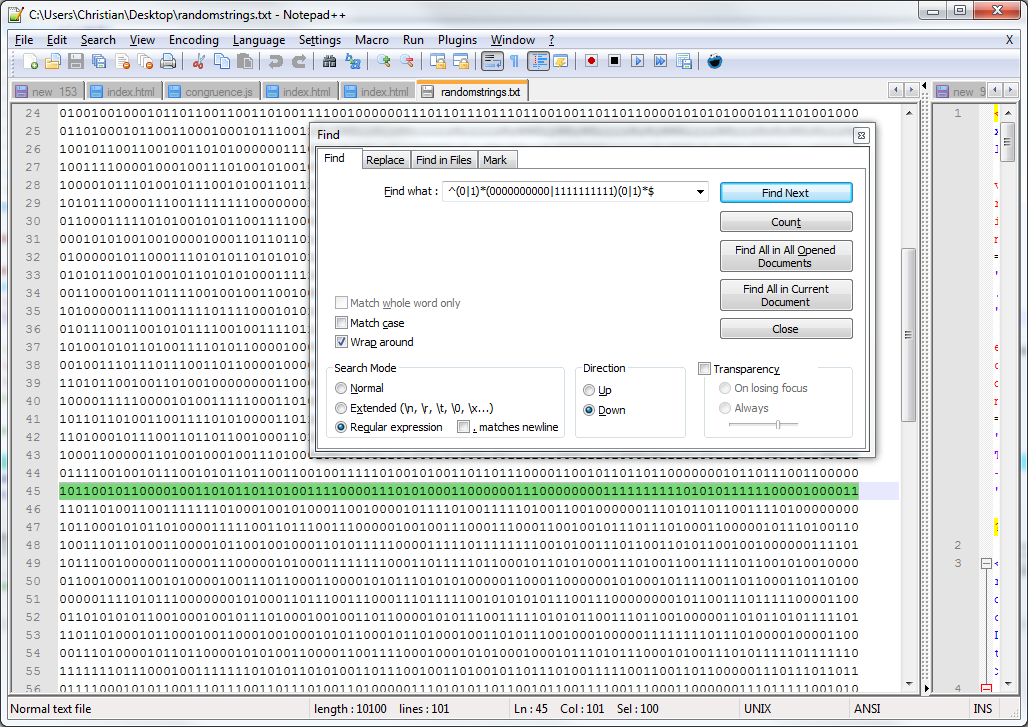
\includegraphics[width=\textwidth]{screenshot.png}
	\end{enumerate}
\end{document}
